\documentclass[twoside]{book}

% Packages required by doxygen
\usepackage{fixltx2e}
\usepackage{calc}
\usepackage{doxygen}
\usepackage[export]{adjustbox} % also loads graphicx
\usepackage{graphicx}
\usepackage[utf8]{inputenc}
\usepackage{makeidx}
\usepackage{multicol}
\usepackage{multirow}
\PassOptionsToPackage{warn}{textcomp}
\usepackage{textcomp}
\usepackage[nointegrals]{wasysym}
\usepackage[table]{xcolor}

% Font selection
\usepackage[T1]{fontenc}
\usepackage[scaled=.90]{helvet}
\usepackage{courier}
\usepackage{amssymb}
\usepackage{sectsty}
\renewcommand{\familydefault}{\sfdefault}
\allsectionsfont{%
  \fontseries{bc}\selectfont%
  \color{darkgray}%
}
\renewcommand{\DoxyLabelFont}{%
  \fontseries{bc}\selectfont%
  \color{darkgray}%
}
\newcommand{\+}{\discretionary{\mbox{\scriptsize$\hookleftarrow$}}{}{}}

% Page & text layout
\usepackage{geometry}
\geometry{%
  a4paper,%
  top=2.5cm,%
  bottom=2.5cm,%
  left=2.5cm,%
  right=2.5cm%
}
\tolerance=750
\hfuzz=15pt
\hbadness=750
\setlength{\emergencystretch}{15pt}
\setlength{\parindent}{0cm}
\setlength{\parskip}{3ex plus 2ex minus 2ex}
\makeatletter
\renewcommand{\paragraph}{%
  \@startsection{paragraph}{4}{0ex}{-1.0ex}{1.0ex}{%
    \normalfont\normalsize\bfseries\SS@parafont%
  }%
}
\renewcommand{\subparagraph}{%
  \@startsection{subparagraph}{5}{0ex}{-1.0ex}{1.0ex}{%
    \normalfont\normalsize\bfseries\SS@subparafont%
  }%
}
\makeatother

% Headers & footers
\usepackage{fancyhdr}
\pagestyle{fancyplain}
\fancyhead[LE]{\fancyplain{}{\bfseries\thepage}}
\fancyhead[CE]{\fancyplain{}{}}
\fancyhead[RE]{\fancyplain{}{\bfseries\leftmark}}
\fancyhead[LO]{\fancyplain{}{\bfseries\rightmark}}
\fancyhead[CO]{\fancyplain{}{}}
\fancyhead[RO]{\fancyplain{}{\bfseries\thepage}}
\fancyfoot[LE]{\fancyplain{}{}}
\fancyfoot[CE]{\fancyplain{}{}}
\fancyfoot[RE]{\fancyplain{}{\bfseries\scriptsize Generated by Doxygen }}
\fancyfoot[LO]{\fancyplain{}{\bfseries\scriptsize Generated by Doxygen }}
\fancyfoot[CO]{\fancyplain{}{}}
\fancyfoot[RO]{\fancyplain{}{}}
\renewcommand{\footrulewidth}{0.4pt}
\renewcommand{\chaptermark}[1]{%
  \markboth{#1}{}%
}
\renewcommand{\sectionmark}[1]{%
  \markright{\thesection\ #1}%
}

% Indices & bibliography
\usepackage{natbib}
\usepackage[titles]{tocloft}
\setcounter{tocdepth}{3}
\setcounter{secnumdepth}{5}
\makeindex

% Hyperlinks (required, but should be loaded last)
\usepackage{ifpdf}
\ifpdf
  \usepackage[pdftex,pagebackref=true]{hyperref}
\else
  \usepackage[ps2pdf,pagebackref=true]{hyperref}
\fi
\hypersetup{%
  colorlinks=true,%
  linkcolor=blue,%
  citecolor=blue,%
  unicode%
}

% Custom commands
\newcommand{\clearemptydoublepage}{%
  \newpage{\pagestyle{empty}\cleardoublepage}%
}

\usepackage{caption}
\captionsetup{labelsep=space,justification=centering,font={bf},singlelinecheck=off,skip=4pt,position=top}

%===== C O N T E N T S =====

\begin{document}

% Titlepage & ToC
\hypersetup{pageanchor=false,
             bookmarksnumbered=true,
             pdfencoding=unicode
            }
\pagenumbering{alph}
\begin{titlepage}
\vspace*{7cm}
\begin{center}%
{\Large Meteologica server }\\
\vspace*{1cm}
{\large Generated by Doxygen 1.8.13}\\
\end{center}
\end{titlepage}
\clearemptydoublepage
\pagenumbering{roman}
\tableofcontents
\clearemptydoublepage
\pagenumbering{arabic}
\hypersetup{pageanchor=true}

%--- Begin generated contents ---
\chapter{Hierarchical Index}
\section{Class Hierarchy}
This inheritance list is sorted roughly, but not completely, alphabetically\+:\begin{DoxyCompactList}
\item \contentsline{section}{Cache$<$ Key, Value $>$}{\pageref{classCache}}{}
\item \contentsline{section}{Cache$<$ std\+:\+:string, std\+:\+:string $>$}{\pageref{classCache}}{}
\item \contentsline{section}{Server}{\pageref{classServer}}{}
\item \contentsline{section}{Socket}{\pageref{classSocket}}{}
\begin{DoxyCompactList}
\item \contentsline{section}{Binding\+Socket}{\pageref{classBindingSocket}}{}
\end{DoxyCompactList}
\item \contentsline{section}{Thread\+Pool}{\pageref{classThreadPool}}{}
\begin{DoxyCompactList}
\item \contentsline{section}{Server\+Thread\+Pool}{\pageref{classServerThreadPool}}{}
\end{DoxyCompactList}
\end{DoxyCompactList}

\chapter{Class Index}
\section{Class List}
Here are the classes, structs, unions and interfaces with brief descriptions\+:\begin{DoxyCompactList}
\item\contentsline{section}{\hyperlink{classBindingSocket}{Binding\+Socket} }{\pageref{classBindingSocket}}{}
\item\contentsline{section}{\hyperlink{classCache}{Cache$<$ Key, Value $>$} }{\pageref{classCache}}{}
\item\contentsline{section}{\hyperlink{classServer}{Server} }{\pageref{classServer}}{}
\item\contentsline{section}{\hyperlink{classServerThreadPool}{Server\+Thread\+Pool} }{\pageref{classServerThreadPool}}{}
\item\contentsline{section}{\hyperlink{classSocket}{Socket} }{\pageref{classSocket}}{}
\item\contentsline{section}{\hyperlink{classThreadPool}{Thread\+Pool} }{\pageref{classThreadPool}}{}
\end{DoxyCompactList}

\chapter{Class Documentation}
\hypertarget{classBindingSocket}{}\section{Binding\+Socket Class Reference}
\label{classBindingSocket}\index{Binding\+Socket@{Binding\+Socket}}


{\ttfamily \#include $<$Binding\+Socket.\+hpp$>$}



Inheritance diagram for Binding\+Socket\+:\nopagebreak
\begin{figure}[H]
\begin{center}
\leavevmode
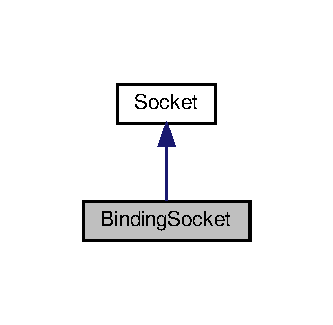
\includegraphics[width=160pt]{classBindingSocket__inherit__graph}
\end{center}
\end{figure}


Collaboration diagram for Binding\+Socket\+:\nopagebreak
\begin{figure}[H]
\begin{center}
\leavevmode
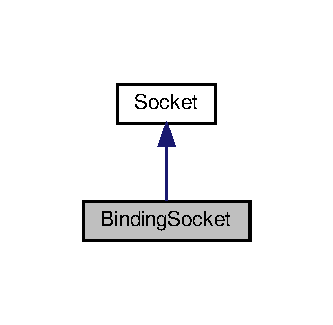
\includegraphics[width=160pt]{classBindingSocket__coll__graph}
\end{center}
\end{figure}
\subsection*{Public Member Functions}
\begin{DoxyCompactItemize}
\item 
\hyperlink{classBindingSocket_aee27b67c01411fa363865e92310b015c}{Binding\+Socket} (int domain, int service, int protocol, int port, u\+\_\+long interface, int bklg)
\begin{DoxyCompactList}\small\item\em Binding (server side) socket constructor. For more information, check \href{https://man7.org/linux/man-pages/man2/socket.2.html}{\tt https\+://man7.\+org/linux/man-\/pages/man2/socket.\+2.\+html}. \end{DoxyCompactList}\item 
int \hyperlink{classBindingSocket_a02a8a46a6a5d5c3205d53f2a9840455a}{connect\+\_\+to\+\_\+network} (int sock, struct sockaddr\+\_\+in address)
\begin{DoxyCompactList}\small\item\em Implements the connection to the network using the bind function. \end{DoxyCompactList}\item 
\mbox{\Hypertarget{classBindingSocket_add8fecb2aa76c3c81bb65861973c487a}\label{classBindingSocket_add8fecb2aa76c3c81bb65861973c487a}} 
void \hyperlink{classBindingSocket_add8fecb2aa76c3c81bb65861973c487a}{start\+\_\+listening} ()
\begin{DoxyCompactList}\small\item\em Function to be called to start listening to the previously specified port. \end{DoxyCompactList}\item 
\mbox{\Hypertarget{classBindingSocket_a76086880c62746d2247befee6a3fe68f}\label{classBindingSocket_a76086880c62746d2247befee6a3fe68f}} 
void \hyperlink{classBindingSocket_a76086880c62746d2247befee6a3fe68f}{test\+\_\+connection} ()
\begin{DoxyCompactList}\small\item\em Test function for the connection. \end{DoxyCompactList}\item 
\mbox{\Hypertarget{classBindingSocket_aa24ab4e79fd3b30b415b3e96eae14a83}\label{classBindingSocket_aa24ab4e79fd3b30b415b3e96eae14a83}} 
void \hyperlink{classBindingSocket_aa24ab4e79fd3b30b415b3e96eae14a83}{test\+\_\+listening} ()
\begin{DoxyCompactList}\small\item\em Test function for the port listening. \end{DoxyCompactList}\item 
\mbox{\Hypertarget{classBindingSocket_acaf64a54e51eea07f5f7268b805ab3d0}\label{classBindingSocket_acaf64a54e51eea07f5f7268b805ab3d0}} 
int \hyperlink{classBindingSocket_acaf64a54e51eea07f5f7268b805ab3d0}{get\+\_\+connection} ()
\begin{DoxyCompactList}\small\item\em Getter for the connection binding, 0 on success, -\/1 on failure. \end{DoxyCompactList}\item 
\mbox{\Hypertarget{classBindingSocket_a562609b198ba3db277549ae4d465d1c2}\label{classBindingSocket_a562609b198ba3db277549ae4d465d1c2}} 
int \hyperlink{classBindingSocket_a562609b198ba3db277549ae4d465d1c2}{get\+\_\+listening} ()
\begin{DoxyCompactList}\small\item\em Getter for the listening, 0 on success, -\/1 on failure. \end{DoxyCompactList}\end{DoxyCompactItemize}


\subsection{Detailed Description}
Binding socket class. It inherits from the generic socket and implements the binding process, used in the server side. 

\subsection{Constructor \& Destructor Documentation}
\mbox{\Hypertarget{classBindingSocket_aee27b67c01411fa363865e92310b015c}\label{classBindingSocket_aee27b67c01411fa363865e92310b015c}} 
\index{Binding\+Socket@{Binding\+Socket}!Binding\+Socket@{Binding\+Socket}}
\index{Binding\+Socket@{Binding\+Socket}!Binding\+Socket@{Binding\+Socket}}
\subsubsection{\texorpdfstring{Binding\+Socket()}{BindingSocket()}}
{\footnotesize\ttfamily Binding\+Socket\+::\+Binding\+Socket (\begin{DoxyParamCaption}\item[{int}]{domain,  }\item[{int}]{service,  }\item[{int}]{protocol,  }\item[{int}]{port,  }\item[{u\+\_\+long}]{interface,  }\item[{int}]{bklg }\end{DoxyParamCaption})}



Binding (server side) socket constructor. For more information, check \href{https://man7.org/linux/man-pages/man2/socket.2.html}{\tt https\+://man7.\+org/linux/man-\/pages/man2/socket.\+2.\+html}. 


\begin{DoxyParams}{Parameters}
{\em domain} & specifies the communicantion domain \\
\hline
{\em service} & specifies the communication semantics \\
\hline
{\em protocol} & specifies a particular protocol to be used with the socket \\
\hline
{\em port} & specifies the number of port that will be used \\
\hline
{\em interface} & specifies port interface \\
\hline
{\em bklg} & defines the maximum length to which the queue of pending connections may grow \\
\hline
\end{DoxyParams}


\subsection{Member Function Documentation}
\mbox{\Hypertarget{classBindingSocket_a02a8a46a6a5d5c3205d53f2a9840455a}\label{classBindingSocket_a02a8a46a6a5d5c3205d53f2a9840455a}} 
\index{Binding\+Socket@{Binding\+Socket}!connect\+\_\+to\+\_\+network@{connect\+\_\+to\+\_\+network}}
\index{connect\+\_\+to\+\_\+network@{connect\+\_\+to\+\_\+network}!Binding\+Socket@{Binding\+Socket}}
\subsubsection{\texorpdfstring{connect\+\_\+to\+\_\+network()}{connect\_to\_network()}}
{\footnotesize\ttfamily int Binding\+Socket\+::connect\+\_\+to\+\_\+network (\begin{DoxyParamCaption}\item[{int}]{sock,  }\item[{struct sockaddr\+\_\+in}]{address }\end{DoxyParamCaption})\hspace{0.3cm}{\ttfamily [virtual]}}



Implements the connection to the network using the bind function. 


\begin{DoxyParams}{Parameters}
{\em sock} & specifies the socket file descriptor for the connection \\
\hline
{\em service} & address specifies the adress struct for the connection \\
\hline
\end{DoxyParams}


Implements \hyperlink{classSocket_a2483ca0900b0d55cfeb4b6cf5724c1e7}{Socket}.



The documentation for this class was generated from the following files\+:\begin{DoxyCompactItemize}
\item 
Binding\+Socket.\+hpp\item 
Binding\+Socket.\+cpp\end{DoxyCompactItemize}

\hypertarget{classCache}{}\section{Cache$<$ Key, Value $>$ Class Template Reference}
\label{classCache}\index{Cache$<$ Key, Value $>$@{Cache$<$ Key, Value $>$}}


{\ttfamily \#include $<$Cache.\+hpp$>$}

\subsection*{Public Types}
\begin{DoxyCompactItemize}
\item 
\mbox{\Hypertarget{classCache_aba9c0839c657c50ce9147b298278dab9}\label{classCache_aba9c0839c657c50ce9147b298278dab9}} 
using {\bfseries value\+\_\+type} = typename std\+::pair$<$ Key, Value $>$
\item 
\mbox{\Hypertarget{classCache_ae0ecf3d225e5d7ee2b9fbf048727609b}\label{classCache_ae0ecf3d225e5d7ee2b9fbf048727609b}} 
using {\bfseries value\+\_\+it} = typename std\+::list$<$ value\+\_\+type $>$\+::iterator
\item 
\mbox{\Hypertarget{classCache_a6af783ab93cfb837dde67795cd99a017}\label{classCache_a6af783ab93cfb837dde67795cd99a017}} 
using {\bfseries operation\+\_\+guard} = typename std\+::lock\+\_\+guard$<$ std\+::mutex $>$
\end{DoxyCompactItemize}
\subsection*{Public Member Functions}
\begin{DoxyCompactItemize}
\item 
\hyperlink{classCache_aff01185fbb5b12ac5e139444e092b471}{Cache} (size\+\_\+t max\+\_\+size)
\begin{DoxyCompactList}\small\item\em \hyperlink{classCache}{Cache} constructor. \end{DoxyCompactList}\item 
void \hyperlink{classCache_a7b54629fb513d4b1652951bb713a0635}{put} (const Key \&key, const Value \&value)
\begin{DoxyCompactList}\small\item\em Puts a key and its value in the cache. \end{DoxyCompactList}\item 
Value \& \hyperlink{classCache_ae2c5a764bec9cf7bcc455d37377ff477}{get} (const Key \&key)
\begin{DoxyCompactList}\small\item\em Queries a value from the cache. \end{DoxyCompactList}\item 
bool \hyperlink{classCache_a3cbee30a98148ba6e15e28e4e096d995}{exists} (const Key \&key)
\begin{DoxyCompactList}\small\item\em Queries if a value is in the cache. \end{DoxyCompactList}\item 
\mbox{\Hypertarget{classCache_a6b13a48d9bc1217c9408e66543655e67}\label{classCache_a6b13a48d9bc1217c9408e66543655e67}} 
size\+\_\+t \hyperlink{classCache_a6b13a48d9bc1217c9408e66543655e67}{Size} ()
\begin{DoxyCompactList}\small\item\em Queries the current size of the cache. \end{DoxyCompactList}\item 
\mbox{\Hypertarget{classCache_addfc9aa7e42dcac6ab1ba103a75cdc66}\label{classCache_addfc9aa7e42dcac6ab1ba103a75cdc66}} 
void \hyperlink{classCache_addfc9aa7e42dcac6ab1ba103a75cdc66}{clear} ()
\begin{DoxyCompactList}\small\item\em Clears the cache. \end{DoxyCompactList}\end{DoxyCompactItemize}
\subsection*{Friends}
\begin{DoxyCompactItemize}
\item 
\mbox{\Hypertarget{classCache_a11049cc49065d8bad3f6154e155922f1}\label{classCache_a11049cc49065d8bad3f6154e155922f1}} 
std\+::ostream \& \hyperlink{classCache_a11049cc49065d8bad3f6154e155922f1}{operator$<$$<$} (std\+::ostream \&os, const \hyperlink{classCache}{Cache} \&c)
\begin{DoxyCompactList}\small\item\em Output operator. Writes the cache content. \end{DoxyCompactList}\end{DoxyCompactItemize}


\subsection{Detailed Description}
\subsubsection*{template$<$typename Key, typename Value$>$\newline
class Cache$<$ Key, Value $>$}

Least recently used cache class. A template class to be used with any types. For more information check \href{https://en.wikipedia.org/wiki/Cache_replacement_policies#Least_recently_used_(LRU)}{\tt https\+://en.\+wikipedia.\+org/wiki/\+Cache\+\_\+replacement\+\_\+policies\#\+Least\+\_\+recently\+\_\+used\+\_\+(\+L\+R\+U)} 

\subsection{Constructor \& Destructor Documentation}
\mbox{\Hypertarget{classCache_aff01185fbb5b12ac5e139444e092b471}\label{classCache_aff01185fbb5b12ac5e139444e092b471}} 
\index{Cache@{Cache}!Cache@{Cache}}
\index{Cache@{Cache}!Cache@{Cache}}
\subsubsection{\texorpdfstring{Cache()}{Cache()}}
{\footnotesize\ttfamily template$<$typename Key, typename Value$>$ \\
\hyperlink{classCache}{Cache}$<$ Key, Value $>$\+::\hyperlink{classCache}{Cache} (\begin{DoxyParamCaption}\item[{size\+\_\+t}]{max\+\_\+size }\end{DoxyParamCaption})\hspace{0.3cm}{\ttfamily [inline]}}



\hyperlink{classCache}{Cache} constructor. 


\begin{DoxyParams}{Parameters}
{\em max\+\_\+size} & specifies the maximum size of the cache. If 0, the cache size will be the maximum posible. \\
\hline
\end{DoxyParams}


\subsection{Member Function Documentation}
\mbox{\Hypertarget{classCache_a3cbee30a98148ba6e15e28e4e096d995}\label{classCache_a3cbee30a98148ba6e15e28e4e096d995}} 
\index{Cache@{Cache}!exists@{exists}}
\index{exists@{exists}!Cache@{Cache}}
\subsubsection{\texorpdfstring{exists()}{exists()}}
{\footnotesize\ttfamily template$<$typename Key, typename Value$>$ \\
bool \hyperlink{classCache}{Cache}$<$ Key, Value $>$\+::exists (\begin{DoxyParamCaption}\item[{const Key \&}]{key }\end{DoxyParamCaption})\hspace{0.3cm}{\ttfamily [inline]}}



Queries if a value is in the cache. 


\begin{DoxyParams}{Parameters}
{\em key} & specifies the key to be queried \\
\hline
\end{DoxyParams}
\mbox{\Hypertarget{classCache_ae2c5a764bec9cf7bcc455d37377ff477}\label{classCache_ae2c5a764bec9cf7bcc455d37377ff477}} 
\index{Cache@{Cache}!get@{get}}
\index{get@{get}!Cache@{Cache}}
\subsubsection{\texorpdfstring{get()}{get()}}
{\footnotesize\ttfamily template$<$typename Key, typename Value$>$ \\
Value\& \hyperlink{classCache}{Cache}$<$ Key, Value $>$\+::get (\begin{DoxyParamCaption}\item[{const Key \&}]{key }\end{DoxyParamCaption})\hspace{0.3cm}{\ttfamily [inline]}}



Queries a value from the cache. 


\begin{DoxyParams}{Parameters}
{\em key} & specifies the key to be queried \\
\hline
\end{DoxyParams}
\mbox{\Hypertarget{classCache_a7b54629fb513d4b1652951bb713a0635}\label{classCache_a7b54629fb513d4b1652951bb713a0635}} 
\index{Cache@{Cache}!put@{put}}
\index{put@{put}!Cache@{Cache}}
\subsubsection{\texorpdfstring{put()}{put()}}
{\footnotesize\ttfamily template$<$typename Key, typename Value$>$ \\
void \hyperlink{classCache}{Cache}$<$ Key, Value $>$\+::put (\begin{DoxyParamCaption}\item[{const Key \&}]{key,  }\item[{const Value \&}]{value }\end{DoxyParamCaption})\hspace{0.3cm}{\ttfamily [inline]}}



Puts a key and its value in the cache. 


\begin{DoxyParams}{Parameters}
{\em key} & specifies the key to be inserted \\
\hline
{\em value} & specifies the value to be inserted \\
\hline
\end{DoxyParams}


The documentation for this class was generated from the following file\+:\begin{DoxyCompactItemize}
\item 
Cache.\+hpp\end{DoxyCompactItemize}

\hypertarget{classServer}{}\section{Server Class Reference}
\label{classServer}\index{Server@{Server}}


{\ttfamily \#include $<$Server.\+hpp$>$}

\subsection*{Public Member Functions}
\begin{DoxyCompactItemize}
\item 
\hyperlink{classServer_abc46ac7076bfd95da8b3b3bf73e687f7}{Server} (int domain, int service, int protocol, int port, u\+\_\+long interface, int bklg, std\+::size\+\_\+t cache\+\_\+size)
\begin{DoxyCompactList}\small\item\em \hyperlink{classServer}{Server} constructor. \end{DoxyCompactList}\item 
\mbox{\Hypertarget{classServer_a4b3aa2579cb1c8cd1d069582c14d0fa6}\label{classServer_a4b3aa2579cb1c8cd1d069582c14d0fa6}} 
\hyperlink{classServer_a4b3aa2579cb1c8cd1d069582c14d0fa6}{$\sim$\+Server} ()
\begin{DoxyCompactList}\small\item\em \hyperlink{classServer}{Server} destructor. \end{DoxyCompactList}\end{DoxyCompactItemize}
\subsection*{Friends}
\begin{DoxyCompactItemize}
\item 
\mbox{\Hypertarget{classServer_ae57da46723e205970eb7acde627edb19}\label{classServer_ae57da46723e205970eb7acde627edb19}} 
class {\bfseries Server\+Thread\+Pool}
\end{DoxyCompactItemize}


\subsection{Detailed Description}
\hyperlink{classServer}{Server} class that manages the connection to the socket and the tasks received 

\subsection{Constructor \& Destructor Documentation}
\mbox{\Hypertarget{classServer_abc46ac7076bfd95da8b3b3bf73e687f7}\label{classServer_abc46ac7076bfd95da8b3b3bf73e687f7}} 
\index{Server@{Server}!Server@{Server}}
\index{Server@{Server}!Server@{Server}}
\subsubsection{\texorpdfstring{Server()}{Server()}}
{\footnotesize\ttfamily Server\+::\+Server (\begin{DoxyParamCaption}\item[{int}]{domain,  }\item[{int}]{service,  }\item[{int}]{protocol,  }\item[{int}]{port,  }\item[{u\+\_\+long}]{interface,  }\item[{int}]{bklg,  }\item[{std\+::size\+\_\+t}]{cache\+\_\+size }\end{DoxyParamCaption})}



\hyperlink{classServer}{Server} constructor. 


\begin{DoxyParams}{Parameters}
{\em domain} & specifies the communicantion domain for the socket \\
\hline
{\em service} & specifies the communication semantics for the socket \\
\hline
{\em protocol} & specifies a particular protocol to be used with the socket \\
\hline
{\em port} & specifies the number of port that will be used for the socket \\
\hline
{\em interface} & specifies port interface for the socket \\
\hline
{\em bklg} & defines the maximum length to which the queue of pending connections may grow in the socket \\
\hline
{\em cache\+\_\+size} & defines the size of the cache \\
\hline
\end{DoxyParams}


The documentation for this class was generated from the following files\+:\begin{DoxyCompactItemize}
\item 
Server.\+hpp\item 
Server.\+cpp\end{DoxyCompactItemize}

\hypertarget{classServerThreadPool}{}\section{Server\+Thread\+Pool Class Reference}
\label{classServerThreadPool}\index{Server\+Thread\+Pool@{Server\+Thread\+Pool}}


{\ttfamily \#include $<$Server\+Thread\+Pool.\+hpp$>$}



Inheritance diagram for Server\+Thread\+Pool\+:\nopagebreak
\begin{figure}[H]
\begin{center}
\leavevmode
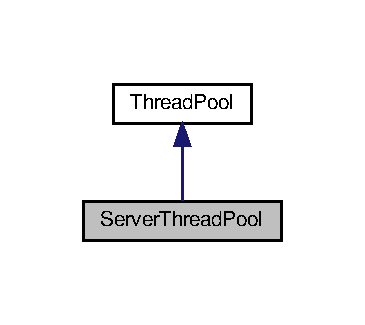
\includegraphics[width=175pt]{classServerThreadPool__inherit__graph}
\end{center}
\end{figure}


Collaboration diagram for Server\+Thread\+Pool\+:\nopagebreak
\begin{figure}[H]
\begin{center}
\leavevmode
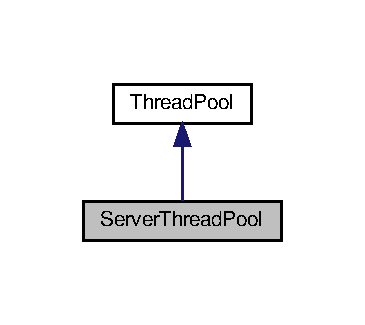
\includegraphics[width=175pt]{classServerThreadPool__coll__graph}
\end{center}
\end{figure}
\subsection*{Public Member Functions}
\begin{DoxyCompactItemize}
\item 
\hyperlink{classServerThreadPool_a2da6753b0170d337851425975763bbf9}{Server\+Thread\+Pool} (std\+::size\+\_\+t cache\+\_\+size)
\begin{DoxyCompactList}\small\item\em \hyperlink{classServer}{Server} thread pool constructor. \end{DoxyCompactList}\item 
\mbox{\Hypertarget{classServerThreadPool_a45205b1fb0646e472e3dbb8bd7a6a9e9}\label{classServerThreadPool_a45205b1fb0646e472e3dbb8bd7a6a9e9}} 
\hyperlink{classServerThreadPool_a45205b1fb0646e472e3dbb8bd7a6a9e9}{$\sim$\+Server\+Thread\+Pool} ()
\begin{DoxyCompactList}\small\item\em \hyperlink{classServer}{Server} thread pool constructor. \end{DoxyCompactList}\item 
\mbox{\Hypertarget{classServerThreadPool_a93e08ed8efb10e755235f6d480f3a37c}\label{classServerThreadPool_a93e08ed8efb10e755235f6d480f3a37c}} 
void \hyperlink{classServerThreadPool_a93e08ed8efb10e755235f6d480f3a37c}{process\+\_\+request} (const std\+::pair$<$ int, std\+::string $>$ request)
\begin{DoxyCompactList}\small\item\em Process requests, returning the M\+D5 hash of the text and sleeping the specified time if the request is valid. \end{DoxyCompactList}\item 
\mbox{\Hypertarget{classServerThreadPool_ad41b2e8022a99e2479020708f50aea39}\label{classServerThreadPool_ad41b2e8022a99e2479020708f50aea39}} 
void \hyperlink{classServerThreadPool_ad41b2e8022a99e2479020708f50aea39}{cache\+\_\+clear} ()
\begin{DoxyCompactList}\small\item\em Clears the cache. \end{DoxyCompactList}\end{DoxyCompactItemize}


\subsection{Detailed Description}
Thread pool class for the implemented server. It does implement the processing of petitions and includes the cache. 

\subsection{Constructor \& Destructor Documentation}
\mbox{\Hypertarget{classServerThreadPool_a2da6753b0170d337851425975763bbf9}\label{classServerThreadPool_a2da6753b0170d337851425975763bbf9}} 
\index{Server\+Thread\+Pool@{Server\+Thread\+Pool}!Server\+Thread\+Pool@{Server\+Thread\+Pool}}
\index{Server\+Thread\+Pool@{Server\+Thread\+Pool}!Server\+Thread\+Pool@{Server\+Thread\+Pool}}
\subsubsection{\texorpdfstring{Server\+Thread\+Pool()}{ServerThreadPool()}}
{\footnotesize\ttfamily Server\+Thread\+Pool\+::\+Server\+Thread\+Pool (\begin{DoxyParamCaption}\item[{std\+::size\+\_\+t}]{cache\+\_\+size }\end{DoxyParamCaption})}



\hyperlink{classServer}{Server} thread pool constructor. 


\begin{DoxyParams}{Parameters}
{\em cache\+\_\+size} & specifies the maximum size of the cache. If 0, the cache size will be the maximum posible. \\
\hline
\end{DoxyParams}


The documentation for this class was generated from the following files\+:\begin{DoxyCompactItemize}
\item 
Server\+Thread\+Pool.\+hpp\item 
Server\+Thread\+Pool.\+cpp\end{DoxyCompactItemize}

\hypertarget{classSocket}{}\section{Socket Class Reference}
\label{classSocket}\index{Socket@{Socket}}


{\ttfamily \#include $<$Socket.\+hpp$>$}



Inheritance diagram for Socket\+:\nopagebreak
\begin{figure}[H]
\begin{center}
\leavevmode
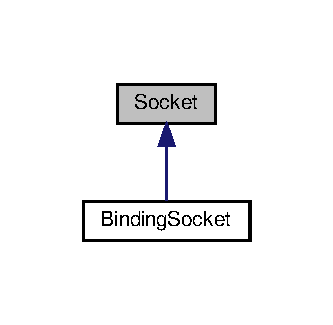
\includegraphics[width=160pt]{classSocket__inherit__graph}
\end{center}
\end{figure}
\subsection*{Public Member Functions}
\begin{DoxyCompactItemize}
\item 
\hyperlink{classSocket_a8be4869e74ddaa7ca8b2a0002fe3ac8e}{Socket} (int domain, int service, int protocol, int port, u\+\_\+long interface)
\begin{DoxyCompactList}\small\item\em \hyperlink{classSocket}{Socket} constructor. For more information, check \href{https://man7.org/linux/man-pages/man2/socket.2.html}{\tt https\+://man7.\+org/linux/man-\/pages/man2/socket.\+2.\+html}. \end{DoxyCompactList}\item 
virtual int \hyperlink{classSocket_a2483ca0900b0d55cfeb4b6cf5724c1e7}{connect\+\_\+to\+\_\+network} (int sock, struct sockaddr\+\_\+in address)=0
\begin{DoxyCompactList}\small\item\em Virtual connection function. Must be implemented as bind (server) or connect (client). \end{DoxyCompactList}\item 
\mbox{\Hypertarget{classSocket_a2a3fd953636d01a796d8b648c785d625}\label{classSocket_a2a3fd953636d01a796d8b648c785d625}} 
void \hyperlink{classSocket_a2a3fd953636d01a796d8b648c785d625}{test\+\_\+sock} ()
\begin{DoxyCompactList}\small\item\em Test function for the socket. \end{DoxyCompactList}\item 
int \hyperlink{classSocket_a134a2436c9fff81048d7815eca284232}{get\+\_\+sock} ()
\begin{DoxyCompactList}\small\item\em Getter function for the socket file descriptor. \end{DoxyCompactList}\item 
struct sockaddr\+\_\+in \hyperlink{classSocket_a6a36bc269e33e3ffda2c224a9b8bf961}{get\+\_\+address} ()
\begin{DoxyCompactList}\small\item\em Getter function for the address struct. \end{DoxyCompactList}\item 
\mbox{\Hypertarget{classSocket_a073b4b728d8b6e366db9caa37a59dbbb}\label{classSocket_a073b4b728d8b6e366db9caa37a59dbbb}} 
virtual \hyperlink{classSocket_a073b4b728d8b6e366db9caa37a59dbbb}{$\sim$\+Socket} ()=default
\begin{DoxyCompactList}\small\item\em Virtual default destructor. \end{DoxyCompactList}\end{DoxyCompactItemize}


\subsection{Detailed Description}
Generic socket class. It does not implement the connection process, as it is different in the server side and in the client side. In this project only the first one will be implemented, but a socket for the client side could also inherit from this class. 

\subsection{Constructor \& Destructor Documentation}
\mbox{\Hypertarget{classSocket_a8be4869e74ddaa7ca8b2a0002fe3ac8e}\label{classSocket_a8be4869e74ddaa7ca8b2a0002fe3ac8e}} 
\index{Socket@{Socket}!Socket@{Socket}}
\index{Socket@{Socket}!Socket@{Socket}}
\subsubsection{\texorpdfstring{Socket()}{Socket()}}
{\footnotesize\ttfamily Socket\+::\+Socket (\begin{DoxyParamCaption}\item[{int}]{domain,  }\item[{int}]{service,  }\item[{int}]{protocol,  }\item[{int}]{port,  }\item[{u\+\_\+long}]{interface }\end{DoxyParamCaption})}



\hyperlink{classSocket}{Socket} constructor. For more information, check \href{https://man7.org/linux/man-pages/man2/socket.2.html}{\tt https\+://man7.\+org/linux/man-\/pages/man2/socket.\+2.\+html}. 


\begin{DoxyParams}{Parameters}
{\em domain} & specifies the communicantion domain \\
\hline
{\em service} & specifies the communication semantics \\
\hline
{\em protocol} & specifies a particular protocol to be used with the socket \\
\hline
{\em port} & specifies the number of port that will be used \\
\hline
{\em interface} & specifies port interface \\
\hline
\end{DoxyParams}


\subsection{Member Function Documentation}
\mbox{\Hypertarget{classSocket_a2483ca0900b0d55cfeb4b6cf5724c1e7}\label{classSocket_a2483ca0900b0d55cfeb4b6cf5724c1e7}} 
\index{Socket@{Socket}!connect\+\_\+to\+\_\+network@{connect\+\_\+to\+\_\+network}}
\index{connect\+\_\+to\+\_\+network@{connect\+\_\+to\+\_\+network}!Socket@{Socket}}
\subsubsection{\texorpdfstring{connect\+\_\+to\+\_\+network()}{connect\_to\_network()}}
{\footnotesize\ttfamily virtual int Socket\+::connect\+\_\+to\+\_\+network (\begin{DoxyParamCaption}\item[{int}]{sock,  }\item[{struct sockaddr\+\_\+in}]{address }\end{DoxyParamCaption})\hspace{0.3cm}{\ttfamily [pure virtual]}}



Virtual connection function. Must be implemented as bind (server) or connect (client). 


\begin{DoxyParams}{Parameters}
{\em sock} & specifies the socket file descriptor for the connection \\
\hline
{\em service} & address specifies the adress struct for the connection \\
\hline
\end{DoxyParams}


Implemented in \hyperlink{classBindingSocket_a02a8a46a6a5d5c3205d53f2a9840455a}{Binding\+Socket}.

\mbox{\Hypertarget{classSocket_a6a36bc269e33e3ffda2c224a9b8bf961}\label{classSocket_a6a36bc269e33e3ffda2c224a9b8bf961}} 
\index{Socket@{Socket}!get\+\_\+address@{get\+\_\+address}}
\index{get\+\_\+address@{get\+\_\+address}!Socket@{Socket}}
\subsubsection{\texorpdfstring{get\+\_\+address()}{get\_address()}}
{\footnotesize\ttfamily struct sockaddr\+\_\+in Socket\+::get\+\_\+address (\begin{DoxyParamCaption}{ }\end{DoxyParamCaption})}



Getter function for the address struct. 

\begin{DoxyReturn}{Returns}
address struct 
\end{DoxyReturn}
\mbox{\Hypertarget{classSocket_a134a2436c9fff81048d7815eca284232}\label{classSocket_a134a2436c9fff81048d7815eca284232}} 
\index{Socket@{Socket}!get\+\_\+sock@{get\+\_\+sock}}
\index{get\+\_\+sock@{get\+\_\+sock}!Socket@{Socket}}
\subsubsection{\texorpdfstring{get\+\_\+sock()}{get\_sock()}}
{\footnotesize\ttfamily int Socket\+::get\+\_\+sock (\begin{DoxyParamCaption}{ }\end{DoxyParamCaption})}



Getter function for the socket file descriptor. 

\begin{DoxyReturn}{Returns}
socket file descriptor 
\end{DoxyReturn}


The documentation for this class was generated from the following files\+:\begin{DoxyCompactItemize}
\item 
Socket.\+hpp\item 
Socket.\+cpp\end{DoxyCompactItemize}

\hypertarget{classThreadPool}{}\section{Thread\+Pool Class Reference}
\label{classThreadPool}\index{Thread\+Pool@{Thread\+Pool}}


{\ttfamily \#include $<$Thread\+Pool.\+hpp$>$}



Inheritance diagram for Thread\+Pool\+:\nopagebreak
\begin{figure}[H]
\begin{center}
\leavevmode
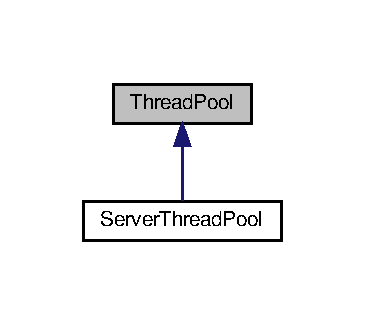
\includegraphics[width=175pt]{classThreadPool__inherit__graph}
\end{center}
\end{figure}
\subsection*{Public Member Functions}
\begin{DoxyCompactItemize}
\item 
\mbox{\Hypertarget{classThreadPool_a3225e86aa7835545b3f6c2c8d363d5e5}\label{classThreadPool_a3225e86aa7835545b3f6c2c8d363d5e5}} 
\hyperlink{classThreadPool_a3225e86aa7835545b3f6c2c8d363d5e5}{Thread\+Pool} ()
\begin{DoxyCompactList}\small\item\em Thread pool constructor. \end{DoxyCompactList}\item 
\mbox{\Hypertarget{classThreadPool_a44d3d2ab618970605e684efc216655eb}\label{classThreadPool_a44d3d2ab618970605e684efc216655eb}} 
\hyperlink{classThreadPool_a44d3d2ab618970605e684efc216655eb}{$\sim$\+Thread\+Pool} ()
\begin{DoxyCompactList}\small\item\em Thread pool destructor. \end{DoxyCompactList}\item 
\mbox{\Hypertarget{classThreadPool_a152a5b1a5ed2274fff48fd03415a4c11}\label{classThreadPool_a152a5b1a5ed2274fff48fd03415a4c11}} 
void \hyperlink{classThreadPool_a152a5b1a5ed2274fff48fd03415a4c11}{queue\+\_\+work} (int fd, std\+::string \&request)
\begin{DoxyCompactList}\small\item\em Add work to the thread pool queue. \end{DoxyCompactList}\end{DoxyCompactItemize}


\subsection{Detailed Description}
Generic thread pool class. It does not implement the processing of the requests. 

The documentation for this class was generated from the following files\+:\begin{DoxyCompactItemize}
\item 
Thread\+Pool.\+hpp\item 
Thread\+Pool.\+cpp\end{DoxyCompactItemize}

%--- End generated contents ---

% Index
\backmatter
\newpage
\phantomsection
\clearemptydoublepage
\addcontentsline{toc}{chapter}{Index}
\printindex

\end{document}
